
\documentclass{article}

\usepackage{pttyr_descriptions}


\begin{document}

\setlist{nolistsep}
\nointerlineskip
\par\noindent
\setlength{\parindent}{0pt}


\section*{Statistics}
\subsection*{\texttt{torch.max}, \texttt{torch.min}}
\prepostc{torch.max(input) or .min}{
  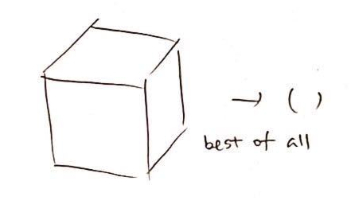
\includegraphics[height=8em]{resources/bestofall.png}
}{}{
  \begin{itemizec}
    \item $|y| = ()$
  \end{itemizec}
}{
  \begin{itemizec}
    \item 주어진 텐서에서 최대/최소 값을 $()$-shape 텐서로 반환(스칼라 X)
  \end{itemizec}
}
\begin{align*}
  \forall \mtt{ft} \in \{\mtt{min}, \mtt{max}\},
  \bigspace
  \frac
  {
    \begin{array}{l}
      \sigma \vdash E \Rar \_, c
    \end{array}
  }
  {
    \sigma \vdash \op{ft}{E} \Rar (), c
  }
\end{align*}

\prepostc{torch.max(input, dim, keep\_dim=False, out=None) or .min}{
  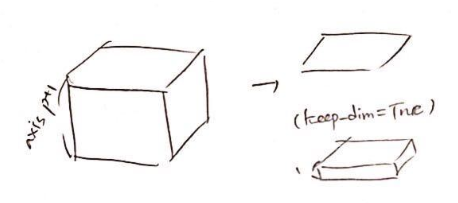
\includegraphics[height=8em]{resources/reduce.png}
}{
  \begin{itemizec}
    \item $|input| = (d_1, d_2, \dots, d_k)$
    \item $k \geq 1$, $0 \leq dim < k$
  \end{itemizec}
}{
  \begin{itemizec}
    \item $|y| = |z| = (d_1, d_2, \dots, d_{dim}, d_{dim+2}, \dots, d_k)$인 $(y,
    z)$ 튜플 반환
    \item 세 번째 인자 $keep\_dim$이 $True$이면 $|y| = |z| = (d_1, d_2, \dots,
    d_{dim}, 1, d_{dim+2}, \dots, d_k)$로 처리
  \end{itemizec}
}{
  \begin{itemizec}
    \item 주어진 텐서에서 축 상의 최대/최소값과, 그에 해당하는 인덱스 번호를
    쌍으로 엮어 튜플로 반환
    \item $out$-텐서 인자가 있는 함수
  \end{itemizec}
}
\begin{align*}
  \forall \mtt{ft} \in \{\mtt{min}, \mtt{max}\},
  \bigspace
  \frac
  {
    \begin{array}{l}
      \sigma \vdash E \Rar e, c \\
      k = \op{rank}{e} \\
      e' = e \indr{1}{n} \conc e \indr{n+2}{k} \\
      c' = \{ (k \geq 1) \land (0 \leq n < k) \}
    \end{array}
  }
  {
    \sigma \vdash \op{ft}{E, n} \Rar (e', e'), c \cup c'
  }
  \tag*{tuple 형태로 반환}
\end{align*}

\begin{align*}
  \forall \mtt{ft} \in \{\mtt{min}, \mtt{max}\},
  \bigspace
  \frac
  {
    \begin{array}{l}
      \sigma \vdash E \Rar e, c \\
      k = \op{rank}{e} \\
      e' = e \indr{1}{n} \conc (1) \conc e \indr{n+2}{k} \\
      c' = \{ (k \geq 1) \land (0 \leq n < k) \}
    \end{array}
  }
  {
    \sigma \vdash \op{ft}{E, n, True} \Rar (e', e'), c \cup c'
  }
  \tag*{tuple 형태로 반환}
\end{align*}

\begin{align*}
  \forall \mtt{ft} \in \{\mtt{min}, \mtt{max}\},
  \bigspace
  \frac
  {
    \sigma \vdash \op{ft}{E, n} \Rar (e, e), c
  }
  {
    \sigma \vdash \op{ft}{E, n, False} \Rar (e, e), c
  }
  \tag*{tuple 형태로 반환}
\end{align*}

\prepostc{torch.max(input, other, out=None) or .min}{
  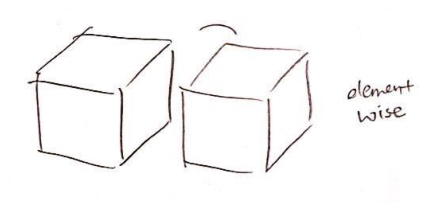
\includegraphics[height=8em]{resources/elementwise.png}
}{
  \begin{itemizec}
    \item $broadcastable(|input|, |other|)$
  \end{itemizec}
}{
  \begin{itemizec}
    \item $broadcast(|input|, |other|)$
  \end{itemizec}
}{
  \begin{itemizec}
    \item 두 텐서의 elementwise 최대/최소
    \item $out$-텐서 인자가 있는 함수
  \end{itemizec}
}
\begin{align*}
  \forall \mtt{ft} \in \{\mtt{min}, \mtt{max}\},
  \bigspace
  \frac
  {
    \begin{array}{l}
      \sigma \vdash E_1 \Rar e_1, c_1 \\
      \sigma \vdash E_2 \Rar e_2, c_2
    \end{array}
  }
  {
    \sigma \vdash \op{ft}{E_1, E_2} \Rar broadcast(e_1, e_2),
      c_1 \cup c_2 \cup broadcastable(e_1, e_2)
  }
\end{align*}

\subsection*{\texttt{torch.sum}, \texttt{torch.mean}}
\prepostc{torch.sum(input, dtype=None) or .mean}{
  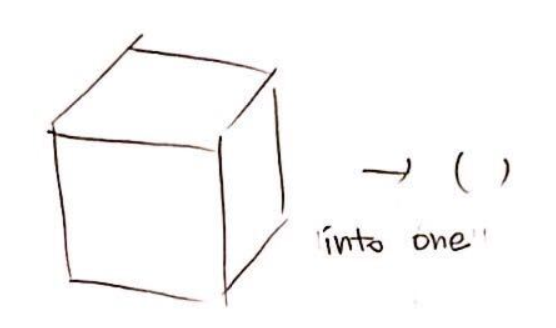
\includegraphics[height=8em]{resources/intoone.png}
}{
  \begin{itemizec}
    \item $\mtt{.mean}$에 대해서는 텐서 타입이 floating이어야 함
  \end{itemizec}
}{
  \begin{itemizec}
    \item $|y| = ()$
  \end{itemizec}
}{
  \begin{itemizec}
    \item 주어진 텐서의 합계/평균값을 $()$-shape 텐서로 반환(스칼라 X)
  \end{itemizec}
}
\begin{align*}
  \forall \mtt{ft} \in \{\mtt{sum}, \mtt{mean}\},
  \bigspace
  \frac
  {
    \begin{array}{l}
      \sigma \vdash E \Rar \_, c
    \end{array}
  }
  {
    \sigma \vdash \op{ft}{E} \Rar (), c
  }
\end{align*}

\prepostc{torch.sum(input, dim, keep\_dim=False, dtype=None) or .mean}{
  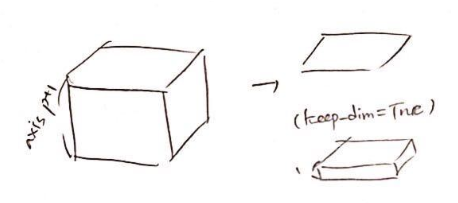
\includegraphics[height=8em]{resources/reduce.png}
}{
  \begin{itemizec}
    \item $|input| = (d_1, d_2, \dots, d_k)$
    \item $k \geq 1$, $0 \leq dim < k$
    \item $\mtt{.mean}$에 대해서는 텐서 타입이 floating이어야 함
  \end{itemizec}
}{
  \begin{itemizec}
    \item $|y| = (d_1, d_2, \dots, d_{dim}, d_{dim+2}, \dots, d_k)$
    \item 세 번째 인자 $keep\_dim$이 $True$이면 $|y| = (d_1, d_2, \dots, d_{dim}, 1,
    d_{dim+2}, \dots, d_k)$
  \end{itemizec}
}{
  \begin{itemizec}
    \item 주어진 텐서에서 축 상의 합/평균을 반환
  \end{itemizec}
}
\begin{align*}
  \forall \mtt{ft} \in \{\mtt{sum}, \mtt{mean}\},
  \bigspace
  \frac
  {
    \begin{array}{l}
      \sigma \vdash E \Rar e, c \\
      k = \op{rank}{e} \\
      e' = e \indr{1}{n} \conc e \indr{n+2}{k} \\
      c' = \{ (k \geq 1) \land (0 \leq n < k) \}
    \end{array}
  }
  {
    \sigma \vdash \op{ft}{E, n} \Rar e', c \cup c'
  }
\end{align*}

\begin{align*}
  \forall \mtt{ft} \in \{\mtt{sum}, \mtt{mean}\},
  \bigspace
  \frac
  {
    \begin{array}{l}
      \sigma \vdash E \Rar e, c \\
      k = \op{rank}{e} \\
      e' = e \indr{1}{n} \conc (1) \conc e \indr{n+2}{k} \\
      c' = \{ (k \geq 1) \land (0 \leq n < k) \}
    \end{array}
  }
  {
    \sigma \vdash \op{ft}{E, n, True} \Rar e', c \cup c'
  }
\end{align*}

\prepostc{torch.sum(input, [n1, n2, ..., nl], keep\_dim=False, dtype=None) or .mean}{
  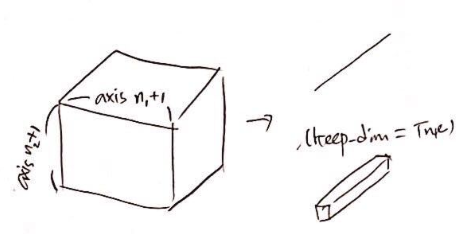
\includegraphics[height=10em]{resources/reduce_multi.png}
}{
  \begin{itemizec}
    \item $|x| = (d_1, d_2, \dots, d_k)$
    \item $k \geq 1$, $0 \leq n_1, n_2, \dots, n_l < k$
    \item $\mtt{.mean}$에 대해서는 텐서 타입이 floating이어야 함
  \end{itemizec}
}{
  \begin{itemizec}
    \item $|y| = (d_{i_1}, d_{i_2}, \dots, d_{i_{k-l}})$
    \begin{itemize}
      \item $1, 2, \dots, k$에서 $n_1+1, n_2+1, \dots, n_l+1$번째 항이 지워진
      shape
    \end{itemize}
    \item 세 번째 인자 $keep\_dim$이 $True$이면 $n_1+1, n_2+1, \dots, n_l+1$번째
    항은 삭제되지 않고 1로 남음
  \end{itemizec}
}{
  \begin{itemizec}
    \item 주어진 텐서에서 여러 축을 통합한 합/평균을 반환
    \item $[n_1, n_2, \dots, n_l]$에 중복된 원소가 들어가도 상관없이 잘 작동함
  \end{itemizec}
}
\begin{align*}
  \forall \mtt{ft} \in \{\mtt{sum}, \mtt{mean}\},
  \bigspace
  \frac
  {
    \begin{array}{l}
      \sigma \vdash E \Rar e, c \\
      k = \op{rank}{e} \\
      e_1 = \ifs{0 \in \{n_1, n_2, \dots, n_r\}}{()}{(e[1])} \\
      e_2 = \ifs{1 \in \{n_1, n_2, \dots, n_r\}}{()}{(e[2])} \\
      \bigspace \cdots \\
      e_k = \ifs{k-1 \in \{n_1, n_2, \dots, n_r\}}{()}{(e[k])} \\
      e' = e_1 \conc e_2 \conc \cdots \conc e_k \\
      c' = \{ (k \geq 1) \land (\forall i=1, 2, \dots, r,\: 0 \leq n_i < k) \}
    \end{array}
  }
  {
    \sigma \vdash \op{ft}{E, (n_1, n_2, \dots, n_r)} \Rar e', c \cup c'
  }
\end{align*}

\begin{align*}
  \forall \mtt{ft} \in \{\mtt{sum}, \mtt{mean}\},
  \bigspace
  \frac
  {
    \begin{array}{l}
      \sigma \vdash E \Rar e, c \\
      k = \op{rank}{e} \\
      e_1 = \ifs{0 \in \{n_1, n_2, \dots, n_r\}}{(1)}{(e[1])} \\
      e_2 = \ifs{1 \in \{n_1, n_2, \dots, n_r\}}{(1)}{(e[2])} \\
      \bigspace \cdots \\
      e_k = \ifs{k-1 \in \{n_1, n_2, \dots, n_r\}}{(1)}{(e[k])} \\
      e' = e_1 \conc e_2 \conc \cdots \conc e_k \\
      c' = \{ (k \geq 1) \land (\forall i=1, 2, \dots, r,\: 0 \leq n_i < k) \}
    \end{array}
  }
  {
    \sigma \vdash \op{ft}{E, (n_1, n_2, \dots, n_r), True} \Rar e', c \cup c'
  }
\end{align*}

\subsection*{\texttt{torch.prod}}
\preposts{torch.prod(input, dtype=None), \\
torch.prod(input, dim, keepdim=False, dtype=None)}{
}{
  \begin{itemizec}
    \item 대부분 \texttt{sum}과 똑같음
    \item 하지만, $dim$ 부분에 튜플값이 들어갈 수 없음. 즉 여러 축에 대한 곱을 계산할 수 없음
  \end{itemizec}
}
\begin{align*}
  \frac
  {
    \begin{array}{l}
      \sigma \vdash E \Rar \_, c
    \end{array}
  }
  {
    \sigma \vdash \op{prod}{E} \Rar (), c
  }
\end{align*}

\begin{align*}
  \frac
  {
    \begin{array}{l}
      \sigma \vdash E \Rar e, c \\
      k = \op{rank}{e} \\
      e' = e \indr{1}{n} \conc e \indr{n+2}{k} \\
      c' = \{ (k \geq 1) \land (0 \leq n < k) \}
    \end{array}
  }
  {
    \sigma \vdash \op{prod}{E, n} \Rar e', c \cup c'
  }
\end{align*}

\begin{align*}
  \frac
  {
    \begin{array}{l}
      \sigma \vdash E \Rar e, c \\
      k = \op{rank}{e} \\
      e' = e \indr{1}{n} \conc (1) \conc e \indr{n+2}{k} \\
      c' = \{ (k \geq 1) \land (0 \leq n < k) \}
    \end{array}
  }
  {
    \sigma \vdash \op{prod}{E, n, True} \Rar e', c \cup c'
  }
\end{align*}

\subsection*{\texttt{torch.Tensor.all}, \texttt{torch.Tensor.any}}
\preposts{a.all(), a.all(dim, keepdim=False, out=None) or .any}{
}{
  \begin{itemizec}
    \item shape의 기능은 \texttt{prod}과 똑같음
    \item \texttt{torch.Tensor} 하위 함수이며, bool-타입 텐서에서만 사용 가능
  \end{itemizec}
}
\begin{align*}
  \forall \mtt{ft} \in \{ \mtt{all}, \mtt{any} \},\bigspace
  \frac
  {
    \begin{array}{l}
      \sigma \vdash E \Rar \_, c
    \end{array}
  }
  {
    \sigma \vdash E.\op{ft}{} \Rar (), c
  }
\end{align*}

\begin{align*}
  \forall \mtt{ft} \in \{ \mtt{all}, \mtt{any} \},\bigspace
  \frac
  {
    \begin{array}{l}
      \sigma \vdash E \Rar e, c \\
      k = \op{rank}{e} \\
      e' = e \indr{1}{n} \conc e \indr{n+2}{k} \\
      c' = \{ (k \geq 1) \land (0 \leq n < k) \}
    \end{array}
  }
  {
    \sigma \vdash E.\op{ft}{n} \Rar e', c \cup c'
  }
\end{align*}

\begin{align*}
  \forall \mtt{ft} \in \{ \mtt{all}, \mtt{any} \},\bigspace
  \frac
  {
    \begin{array}{l}
      \sigma \vdash E \Rar e, c \\
      k = \op{rank}{e} \\
      e' = e \indr{1}{n} \conc (1) \conc e \indr{n+2}{k} \\
      c' = \{ (k \geq 1) \land (0 \leq n < k) \}
    \end{array}
  }
  {
    \sigma \vdash E.\op{ft}{n, True} \Rar e', c \cup c'
  }
\end{align*}


\subsection*{\texttt{torch.var}, \texttt{torch.std}}
\prepostc{torch.var(input, unbiased=True) or .std}{
}{
  \begin{itemizec}
    \item 텐서 타입이 floating이어야 함
  \end{itemizec}
}{
  \begin{itemizec}
    \item $|y| = ()$
  \end{itemizec}
}{
  \begin{itemizec}
    \item 주어진 텐서의 분산/표준편차를 $()$-shape 텐서로 반환(스칼라 X)
  \end{itemizec}
}
\begin{align*}
  \forall \mtt{ft} \in \{\mtt{var}, \mtt{std}\},
  \bigspace
  \frac
  {
    \begin{array}{l}
      \sigma \vdash E \Rar \_, c
    \end{array}
  }
  {
    \sigma \vdash \op{ft}{E} \Rar (), c
  }
\end{align*}

\prepostc{torch.var(input, dim, keepdim=False, unbiased=None, out=None) or \\
torch.std(input, dim, unbiased=True, keepdim=False, out=None)}{
}{
  \begin{itemizec}
    \item $|input| = (d_1, d_2, \dots, d_k)$
    \item $k \geq 1$, $0 \leq dim < k$
    \item 텐서 타입이 floating이어야 함
  \end{itemizec}
}{
  \begin{itemizec}
    \item $|y| = (d_1, d_2, \dots, d_{dim}, d_{dim+2}, \dots, d_k)$
    \item $keepdim$이 $True$이면 $|y| = (d_1, d_2, \dots, d_{dim}, 1,
    d_{dim+2}, \dots, d_k)$
  \end{itemizec}
}{
  \begin{itemizec}
    \item 주어진 텐서에서 축 상의 분산/표준편차를 반환
    \item \texttt{sum}, \texttt{mean}과 마찬가지로 $dim$ 부분은 튜플로 쓰일 수도 있음
    (여러 축에 대한 분산/표춘편차)
  \end{itemizec}
}
\begin{align*}
  \forall \mtt{ft} \in \{\mtt{var}, \mtt{std}\},
  \bigspace
  \frac
  {
    \begin{array}{l}
      \sigma \vdash E \Rar e, c \\
      k = \op{rank}{e} \\
      e' = e \indr{1}{n} \conc e \indr{n+2}{k} \\
      c' = \{ (k \geq 1) \land (0 \leq n < k) \}
    \end{array}
  }
  {
    \sigma \vdash \op{ft}{E, n} \Rar e', c \cup c'
  }
\end{align*}

\begin{align*}
  \forall \mtt{ft} \in \{\mtt{var}, \mtt{std}\},
  \bigspace
  \frac
  {
    \begin{array}{l}
      \sigma \vdash E \Rar e, c \\
      k = \op{rank}{e} \\
      e' = e \indr{1}{n} \conc (1) \conc e \indr{n+2}{k} \\
      c' = \{ (k \geq 1) \land (0 \leq n < k) \}
    \end{array}
  }
  {
    \sigma \vdash \op{ft}{E, n, True} \Rar e', c \cup c'
  }
  \\
  \tag*{$keepdim$이 $True$인 상황에 대한 proof tree}
\end{align*}

\begin{align*}
  \forall \mtt{ft} \in \{\mtt{var}, \mtt{std}\},
  \bigspace
  \frac
  {
    \begin{array}{l}
      \sigma \vdash E \Rar e, c \\
      k = \op{rank}{e} \\
      e_1 = \ifs{0 \in \{n_1, n_2, \dots, n_r\}}{()}{(e[1])} \\
      e_2 = \ifs{1 \in \{n_1, n_2, \dots, n_r\}}{()}{(e[2])} \\
      \bigspace \cdots \\
      e_k = \ifs{k-1 \in \{n_1, n_2, \dots, n_r\}}{()}{(e[k])} \\
      e' = e_1 \conc e_2 \conc \cdots \conc e_k \\
      c' = \{ (k \geq 1) \land (\forall i=1, 2, \dots, r,\: 0 \leq n_i < k) \}
    \end{array}
  }
  {
    \sigma \vdash \op{ft}{E, (n_1, n_2, \dots, n_r)} \Rar e', c \cup c'
  }
\end{align*}

\begin{align*}
  \forall \mtt{ft} \in \{\mtt{var}, \mtt{std}\},
  \bigspace
  \frac
  {
    \begin{array}{l}
      \sigma \vdash E \Rar e, c \\
      k = \op{rank}{e} \\
      e_1 = \ifs{0 \in \{n_1, n_2, \dots, n_r\}}{(1)}{(e[1])} \\
      e_2 = \ifs{1 \in \{n_1, n_2, \dots, n_r\}}{(1)}{(e[2])} \\
      \bigspace \cdots \\
      e_k = \ifs{k-1 \in \{n_1, n_2, \dots, n_r\}}{(1)}{(e[k])} \\
      e' = e_1 \conc e_2 \conc \cdots \conc e_k \\
      c' = \{ (k \geq 1) \land (\forall i=1, 2, \dots, r,\: 0 \leq n_i < k) \}
    \end{array}
  }
  {
    \sigma \vdash \op{ft}{E, (n_1, n_2, \dots, n_r), True} \Rar e', c \cup c'
  }
  \\
  \tag*{$keepdim$이 $True$인 상황에 대한 proof tree}
\end{align*}

\subsection*{\texttt{torch.mode}, \texttt{torch.median}}
\prepostc{torch.mode(input, dim=-1, keep\_dim=False, out=None) or torch.median}{
  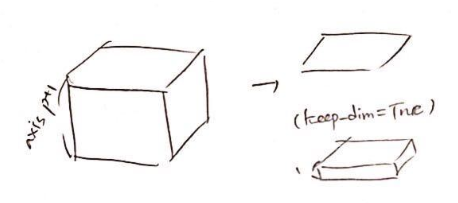
\includegraphics[height=8em]{resources/reduce.png}
}{
  \begin{itemizec}
    \item $|input| = (d_1, d_2, \dots, d_k)$
    \item $k \geq 1$
    \item $0 \leq dim < k$ ($dim \leftarrow k-1$ if $dim = -1$)
  \end{itemizec}
}{
  \begin{itemizec}
    \item $|y| = |z| = (d_1, d_2, \dots, d_{dim}, d_{dim+2}, \dots, d_k)$인 $(y, z)$
    튜플 반환
    \item 세 번째 인자 $keep\_dim$이 $True$이면 $|y| = |z| = (d_1, d_2, \dots,
    d_{dim}, 1, d_{dim+2}, \dots, d_k)$
  \end{itemizec}
}{
  \begin{itemizec}
    \item 입력받은 축을 기준으로한 통계적 최빈값/중간값 계산 함수
    \item (결과값, 인덱스) 튜플 형태로 반환하기 때문에, \texttt{out}인자도
          들어가는 텐서도 2-원소 튜플 형태로 들어감
  \end{itemizec}
}
\begin{align*}
  \forall \mtt{ft} \in \{ \mtt{mode}, \mtt{median} \}, \bigspace
  \frac
  {
    \begin{array}{l}
      \sigma \vdash E \Rar e, c \\
      k = \op{rank}{e} \\
      e' = e \indr{1}{n} \conc e \indr{n+2}{k} \\
      c' = \{ (k \geq 1) \land (0 \leq n < k) \}
    \end{array}
  }
  {
    \sigma \vdash \op{ft}{E, n=-1, out=None} \Rar (e', e'), c \cup c'
  }
  \tag*{tuple 형태로 반환}
\end{align*}

\begin{align*}
  \forall \mtt{ft} \in \{ \mtt{mode}, \mtt{median} \}, \bigspace
  \frac
  {
    \begin{array}{l}
      \sigma \vdash E \Rar e, c \\
      k = \op{rank}{e} \\
      e' = e \indr{1}{n} \conc (1) \conc e \indr{n+2}{k} \\
      c' = \{ (k \geq 1) \land (0 \leq n < k) \}
    \end{array}
  }
  {
    \sigma \vdash \op{ft}{E, n=-1, True, out=None} \Rar (e', e'), c \cup c'
  }
  \tag*{tuple 형태로 반환}
\end{align*}

\begin{align*}
  \forall \mtt{ft} \in \{ \mtt{mode}, \mtt{median} \}, \bigspace
  \frac
  {
    \sigma \vdash \op{ft}{E, n} \Rar (e, e), c
  }
  {
    \sigma \vdash \op{ft}{E, n=-1, False, out=None} \Rar (e, e), c
  }
  \tag*{tuple 형태로 반환}
\end{align*}

\end{document}
